\subsection{Editor Extension Components}\label{sec:extension-components}

This section will describe the most relevant components, libraries or widgets for \acrshort{emf} in the \gls{cloud}, which can be used to create editor extensions.

Some of the libraries belong to \emph{EMF.Cloud}.
That is an Eclipse Foundation project umbrella for \gls{emf} tools for the \gls{cloud}\footnote{Eclipse EMF.cloud homepage: \href{https://projects.eclipse.org/projects/ecd.emfcloud}{https://projects.eclipse.org/projects/ecd.emfcloud}.}.


\subsubsection{Sprotty}\label{sec:sprotty}
Eclipse Sprotty is an \gls{open source}\footnote{Sprotty source: \href{https://github.com/eclipse/sprotty}{https://github.com/eclipse/sprotty}.} library to render diagrams in web browsers.
It uses Typescript, CSS and svg.
Sprotty can animate diagram changes.
The architecture is made with \gls{LSP} in mind, and supports having diagram data sent from a backend.
The library is configurable using dependency injection, and allows for adding custom nodes, edges and behaviors.
It also provides ``glue code'' for easy integration with \gls{LSP}, \gls{Theia} and \gls{ELK}.~\cite{smithEclipseSprotty2018}
An example of a sprotty diagram is shown in \cref{fig:sprotty-example}.

The library is mainly developed by TypeFox and EclipseSource, and managed by the Eclipse Foundation.~\cite{eclipsefoundationEclipseSprotty}

\begin{figure}[htbp]  % order of priority: h here, t top, b bottom, p page
  \centering
  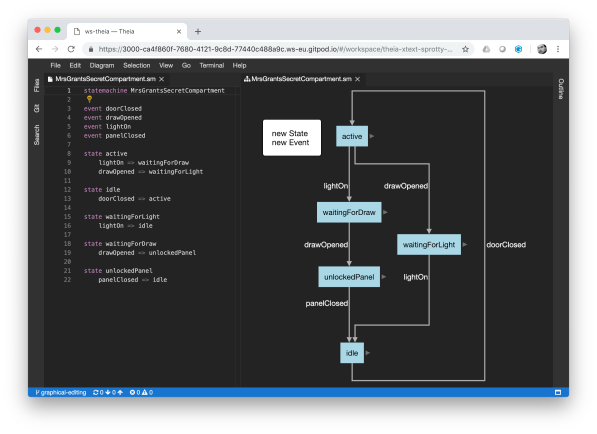
\includegraphics[width=.5\textwidth]{figures/sprotty-example.png}
  \caption[Sprotty Example]{This is a screenshot of Theia with a Sprotty diagram on the right side.~\cite{eclipsefoundationEclipseSprotty2020}}\label{fig:sprotty-example}
\end{figure}

\subsubsection{EMF.Cloud --- Theia Tree Editor}\label{sec:theia-tree-editor}
The \emph{Theia Tree Editor} is an \gls{open source}\footnote{Theia Tree Editor source: \href{https://github.com/eclipse-emfcloud/theia-tree-editor/tree/master/theia-tree-editor}{https://github.com/eclipse-emfcloud/theia-tree-editor/tree/master/theia-tree-editor}.} javascript framework for building tree editors in \gls{Theia}.~\cite{EclipseemfcloudTheiatreeeditor2020}
The framework is targeted at Theia Extensions (see \cref{sec:theia-extension}), and can not probably not be used in \gls{VSCode}\footnote{It \textit{may} be possible, if the VSCode extension pulls in the Theia \texttt{core}, however there could be dependencies to other \gls{Theia} \acrshortpl{API} as well.}.
The main reason is the dependence on tree structures defined in the Theia \acrshort{IDE} project itself (see \cref{fig:theia-tree-editor-node}).
To render the property form, it uses the \emph{JSON-Forms} library (\cref{sec:json-forms}).
Additionally, it uses \gls{React}.

\begin{figure}[htbp]  % order of priority: h here, t top, b bottom, p page
  \centering
  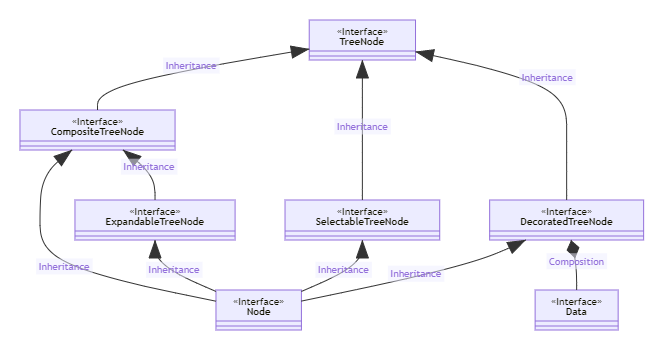
\includegraphics[width=\textwidth]{figures/theia-tree-editor-node.png}
  \caption[Theia Tree Editor Node's Class Hierarchy]{The Node class in Theia Tree Editor inherits multiple interfaces, all from the Theia \texttt{core} extension. Only \texttt{Node} resides in the Theia Tree Editor library itself.}\label{fig:theia-tree-editor-node}
\end{figure}

\subsubsection{JSON-Forms}\label{sec:json-forms}
JSON-Forms is an \gls{open source}\footnote{JSON-Forms source: \href{https://github.com/eclipsesource/jsonforms}{https://github.com/eclipsesource/jsonforms}.} javascript library by EclipseSource for creating HTML form editors.
A form is defined by two key elements: a \emph{data/JSON schema} and a \emph{UI schema}.
The \gls{JSON} schema defines the data types and validations for input.
The User Interface (UI) schema defines the visible \emph{form controls} (text fields, groups, labels) and binds them to a object property in the JSON schema.~\cite{eclipsesourceJSONForms}
For an example of how a form can look like, see \cref{fig:json-forms-example}.

A visual editor for JSON-Forms schemas exist at \href{https://github.com/eclipsesource/jsonforms-editor}{https://github.com/eclipsesource/jsonforms-editor}.

\begin{figure}[htbp]  % order of priority: h here, t top, b bottom, p page
  \centering
  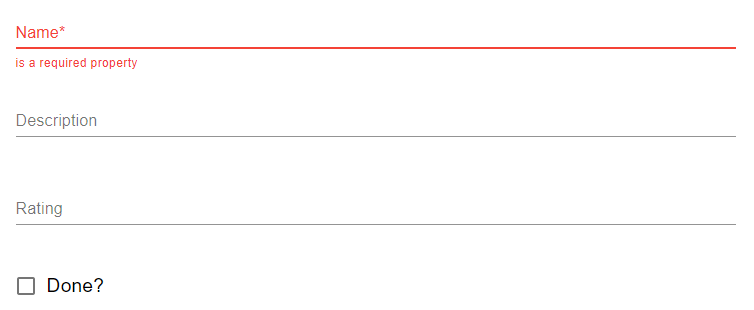
\includegraphics[width=.8\textwidth]{figures/json-forms-example}
  \caption[JSON-Forms Example]{An example of a form generated by JSON-Forms. It is displayed in a web browser.}\label{fig:json-forms-example}
\end{figure}

\subsubsection{EMF.Cloud --- Model Server}
The \emph{Model Server} is an \gls{open source}\footnote{Model Server source: \href{https://github.com/eclipse-emfcloud/emfcloud-modelserver}{https://github.com/eclipse-emfcloud/emfcloud-modelserver}.} java library and standalone web server.
It can discover and read \gls{Ecore} and \gls{XMI} files in a workspace folder.
Then the models can be provided as \gls{JSON} over a \gls{REST} \acrshort{API}, and changes to the models can be provided via \gls{WebSocket} subscriptions.~\cite{eugenneufeldEclipseemfcloudEmfcloudmodelserver2020}

A copy of the standalone \texttt{.jar} can be downloaded from a Maven Repository at \href{https://oss.sonatype.org/content/repositories/snapshots/org/eclipse/emfcloud/modelserver/org.eclipse.emfcloud.modelserver.example/0.7.0-SNAPSHOT/}{https://oss.sonatype.org/content/repositories/snapshots/org/eclipse/emfcloud/modelserver/org.eclipse.emfcloud.modelserver.example/0.7.0-SNAPSHOT/}.
(Note that the standalone seems to embed a coffee model example.
However, the implementation works with all \texttt{EObject}s and reads the \gls{Ecore} metamodel, so the use of the coffee model is not clear).
The \acrshort{API} provided can also serve \emph{JSON-Schema} and \emph{UI Schema}, which JSON-Forms in \cref{sec:json-forms} can consume.

The Model Server could be used in an extension or plugin (\cref{sec:extension-mechanisms}) as a backend child process, provided that the host operating system has a java runtime available.

%\subsubsection{Eclipse Edit} ?
% TODO: write
% From genmodel. Strictly not cloud, but could aid a backend.

\subsubsection{EMF.Cloud --- emfjson-jackson}
Originally, \emph{emfjson} was a project umbrella for \gls{emf} in the \gls{cloud}.
One part of emfjson, the \gls{JSON} serializer called \emph{emfjson-jackson} was donated to EMF.Cloud.
This is an \gls{open source}\footnote{Emfjson-jackson source: \href{https://github.com/eclipse-emfcloud/emfjson-jackson}{https://github.com/eclipse-emfcloud/emfjson-jackson}.} java library which uses the Jackson JSON library.\cite{guillaumehillairetEclipseemfcloudEmfjsonjackson2020}

% ecore.js ?https://github.com/emfjson/ecore.js